\chapter{Temperatuur en thermometers}\label{ch:g3:temperature-thermometers}

Twee winters geleden hielden drie kommen water je twee handen voor de
gek: hetzelfde water voelde warm voor de ene en koel voor de andere.
We beloofden toen dat er ooit een instrument zou komen dat zulke
ruzies beslecht. Hier is het --- de \omterm{def:g3:temperature-thermometers:temperature}{thermometer}, de kleine glazen
rechter die warm en koud in een getal verandert.

\section{Waarom gevoel niet genoeg is}

\begin{example}[De oneerlijke rechters]\label{ex:g3:temperature-thermometers:unfair}
In elk seizoen oordeelt je gevoel oneerlijk: de metalen glijbaan voelt
kouder dan de houten bank in dezelfde \omterm{def:g1:light-and-shadows:shadow}{schaduw}; lauw water voelt warm
voor een koude hand en koel voor een warme; en na het sleeën voelt de
kille gang lekker behaaglijk. Om warm en koud eerlijk te vergelijken
--- van kamer tot kamer, van dag tot dag, van mens tot mens --- hebben
we een rechter nodig die nooit van gedachten verandert: een
instrument.
\end{example}

\section{De thermometer en zijn graden}

\begin{definition}[Temperatuur]\label{def:g3:temperature-thermometers:temperature}
De \emph{temperatuur}\index{temperatuur} van iets is het getal dat
precies zegt hoe warm of koud het is. Hoger getal, warmer ding; lager
getal, kouder ding. Temperatuur wordt gemeten in \emph{graden
Celsius}\index{graad Celsius}, geschreven \unit{\celsius}, met een
\emph{thermometer}\index{thermometer}.
\end{definition}

\begin{proposition}[De twee mijlpalen van water]\label{prop:g3:temperature-thermometers:milestones}
De Celsiusschaal is vastgepind op de twee grote
toestandsveranderingen van water:
\begin{enumerate}
  \item bij \qty{0}{\celsius} \omterm{def:g2:ice-water-steam:meltfreeze}{bevriest} water tot ijs (en \omterm{def:g2:ice-water-steam:meltfreeze}{smelt} ijs);
  \item bij \qty{100}{\celsius} kookt water tot damp.
\end{enumerate}
Tussen de twee mijlpalen is de schaal in $100$ gelijke graden verdeeld
--- een trap van kleinere treden van ijs naar damp.
\end{proposition}

\begin{omfigure}
\begin{tikzpicture}[scale=0.85]
  \draw[thick] (0.5,0) rectangle (1.1,6.0);
  \draw[thick] (0.8,0) circle (0.42);
  \fill[omThm, opacity=0.7] (0.8,0) circle (0.34);
  % scale: 0 C at y=0.6, one unit of height per 20 C -> 25 C at y=1.85
  \fill[omThm, opacity=0.7] (0.62,0.05) rectangle (0.98,1.85);
  \foreach \y/\t in {0.6/0, 1.6/20, 2.6/40, 3.6/60, 4.6/80, 5.6/100} {
    \draw (1.1,\y) -- (1.35,\y);
    \node[right, font=\footnotesize] at (1.4,\y) {$\t$};
  }
  \foreach \y in {1.1, 2.1, 3.1, 4.1, 5.1} {
    \draw (1.1,\y) -- (1.25,\y);
  }
  \node[right, font=\small, omDef] at (2.6,0.6)
    {\qty{0}{\celsius}: water bevriest};
  \node[right, font=\small] at (2.6,1.85)
    {\qty{25}{\celsius}: deze aflezing};
  \node[right, font=\small, omThm] at (2.6,5.6)
    {\qty{100}{\celsius}: water kookt};
  \draw[-Stealth, omExo] (2.5,1.85) -- (1.05,1.85);
\end{tikzpicture}

{\small Een \omterm{def:g3:temperature-thermometers:temperature}{thermometer}: de rode \omterm{def:g3:solids-liquids-gases:liquid}{vloeistof} klimt als ze verwarmd wordt.
Hier staat ze op het streepje $25$ --- de \omterm{def:g3:temperature-thermometers:temperature}{temperatuur} is
\qty{25}{\celsius}.}
\end{omfigure}

\begin{example}[Hoe de glazen rechter werkt]\label{ex:g3:temperature-thermometers:works}
In het dunne buisje van de \omterm{def:g3:temperature-thermometers:temperature}{thermometer} zit een opgesloten gekleurde
\omterm{def:g3:solids-liquids-gases:liquid}{vloeistof}. Warmte laat die \omterm{def:g3:solids-liquids-gases:liquid}{vloeistof} een klein beetje uitzetten --- en in
zo'n dun buisje duwt een kleine uitzetting de kolom zichtbaar omhoog.
Kou laat haar weer krimpen. De \omterm{def:g3:solids-liquids-gases:liquid}{vloeistof} laat zich niet voor de gek
houden zoals een hand: ze zet even veel uit bij dezelfde warmte,
vandaag, morgen, voor iedereen.
\end{example}

\begin{omfigure}
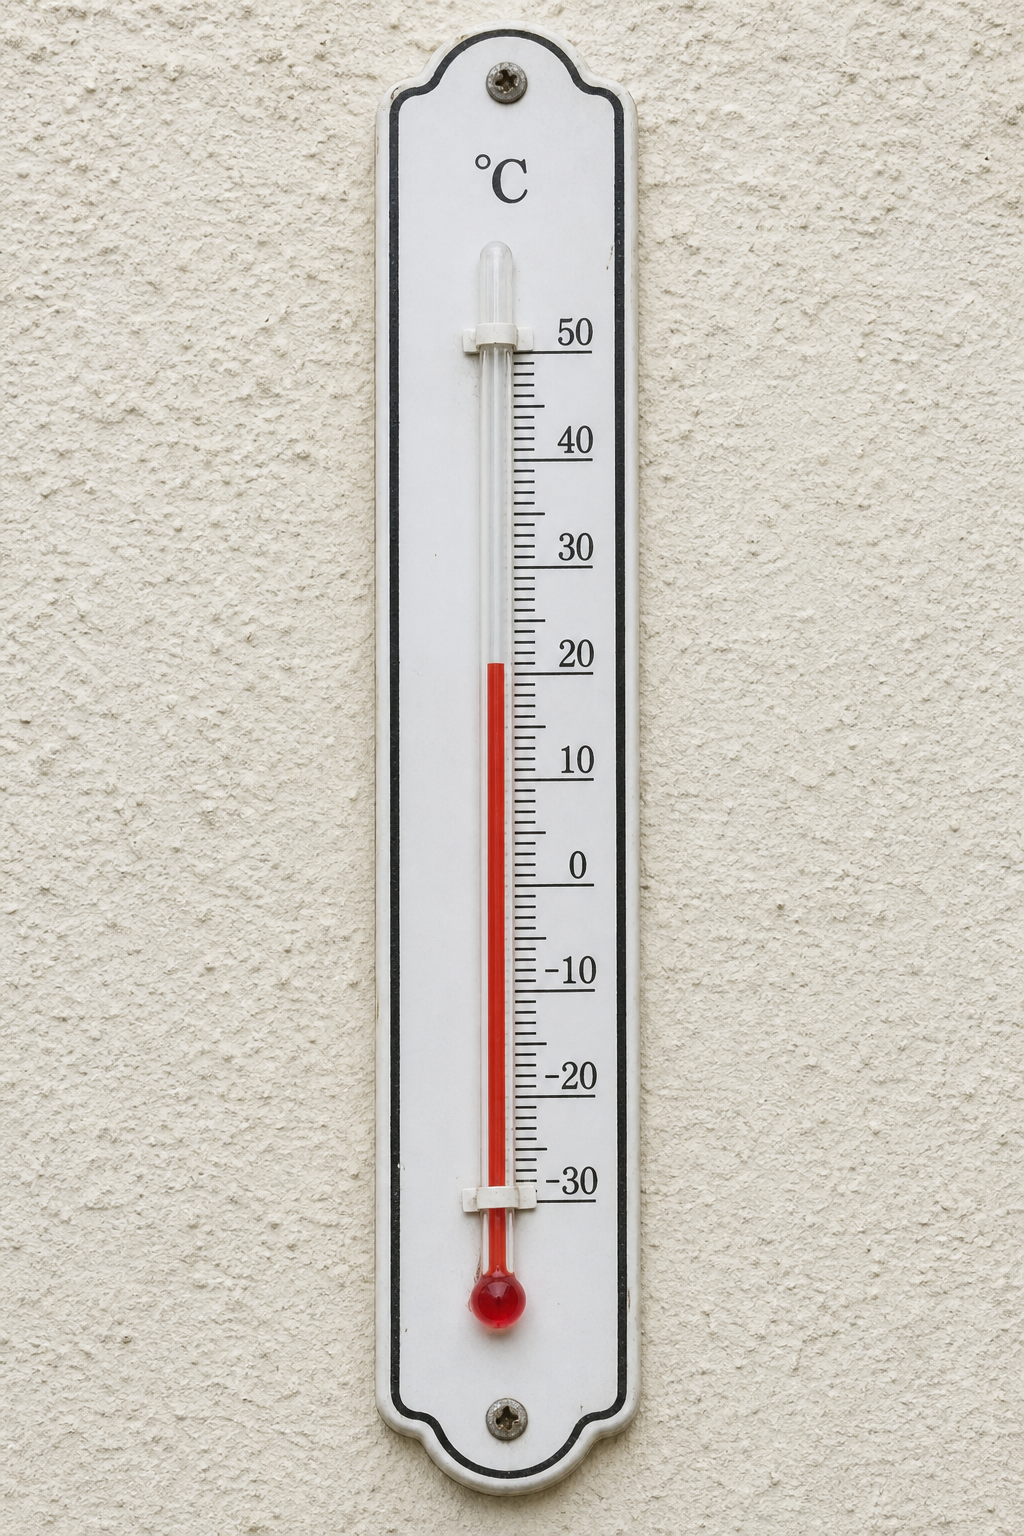
\includegraphics[width=0.3\linewidth]{images/book1/ai/g3-thermometer-outdoor.png}

{\small Een echte \omterm{def:g3:temperature-thermometers:temperature}{thermometer} aan de muur: de rode kolom klimt langs de schaal, en iedereen die het streepje afleest krijgt hetzelfde getal.}
\end{omfigure}

\section{Een thermometer aflezen}

\begin{method}[Een thermometer aflezen]\label{met:g3:temperature-thermometers:read}
\begin{enumerate}
  \item Zet de \omterm{def:g3:temperature-thermometers:temperature}{thermometer} waar je de \omterm{def:g3:temperature-thermometers:temperature}{temperatuur} wilt weten --- in het
        water, buiten in de \omterm{def:g1:light-and-shadows:shadow}{schaduw}, onder de tong;
  \item \emph{wacht} --- de \omterm{def:g3:solids-liquids-gases:liquid}{vloeistof} heeft tijd nodig om uitgeklommen
        of uitgezakt te zijn; kijk tot ze stilstaat;
  \item breng je oog op gelijke hoogte met de bovenkant van de kolom;
  \item lees het getal af bij het streepje waar de kolom komt, en
        schrijf het met zijn \omterm{def:g2:measuring-length:measure}{eenheid}: \qty{18}{\celsius}.
\end{enumerate}
Te vroeg aflezen, of schuin van opzij, geeft een verkeerd getal --- de
rechter is eerlijk, maar je moet hem netjes ondervragen.
\end{method}

\begin{example}[Temperaturen om mee te leven]\label{ex:g3:temperature-thermometers:livedby}
Een paar getallen die je uit je hoofd moet kennen: een aangename kamer
is ongeveer \qty{20}{\celsius}; je lichaam houdt zichzelf op ongeveer
\qty{37}{\celsius}, zomer en winter; ver daarboven is koorts --- de
\omterm{def:g3:temperature-thermometers:temperature}{thermometer} van de dokter weet het. De koelkast houdt ongeveer
\qty{4}{\celsius}; een hete zomerdag haalt \qty{30}{\celsius};
badwater is aangenaam rond \qty{35}{\celsius}.
\end{example}

\begin{omfigure}
\begin{tikzpicture}[scale=0.85]
  \foreach \x/\h/\t/\name in {0/1.1/4/koelkast,
      3.0/2.1/20/een aangename kamer, 6.0/3.0/37/je lichaam,
      9.0/2.6/30/zomerdag} {
    \draw[thick] (\x,0) rectangle ++(0.42,3.6);
    \fill[omThm, opacity=0.7] (\x+0.08,0.05) rectangle ++(0.26,\h);
    \node[above, font=\footnotesize] at (\x+0.21,3.65)
      {$\t$\,\unit{\celsius}};
    \node[below, font=\small, align=center] at (\x+0.21,-0.2) {\name};
  }
\end{tikzpicture}

{\small Vier vertrouwde temperaturen: hoe hoger de kolom, hoe warmer
het ding.}
\end{omfigure}

\section{Onder nul}

\begin{example}[Wintergetallen]\label{ex:g3:temperature-thermometers:belowzero}
Op een vrieskoude ochtend zakt de kolom \emph{onder} het streepje $0$.
De streepjes lopen daar gewoon door, en we lezen ze met het woord
``min'': één streepje onder nul is \emph{min één} graad, vijf
streepjes eronder is \emph{min vijf}, geschreven \qty{-5}{\celsius}.
Mingetallen zijn kouder dan nul, en hoe verder ze zakken, hoe strenger
de vorst: een ochtend van $-10$ bijt kouder dan een van $-2$. Het
weerbericht noemt ze elke winteravond.
\end{example}

\begin{remark}[Nul is niet ``niets'']\label{rem:g3:temperature-thermometers:zero}
Op deze schaal betekent $0$ niet ``geen \omterm{def:g3:temperature-thermometers:temperature}{temperatuur}'' --- het is
gewoon het streepje waar water \omterm{def:g2:ice-water-steam:meltfreeze}{bevriest}, een mijlpaal als een
wegwijzer. Het weer kan warmer zijn dan de mijlpaal of kouder; de
\omterm{def:g3:temperature-thermometers:temperature}{thermometer} vertelt je alleen aan welke kant, en hoeveel streepjes.
(Getallen onder nul hebben een hele eigen rekenkunde --- je
wiskundecursus pakt die in een later jaar netjes op.)
\end{remark}

\section{Oefeningen}

\begin{exercise}[$\star$]\label{exo:g3:temperature-thermometers:1}
Waarom is een \omterm{def:g3:temperature-thermometers:temperature}{thermometer} een eerlijkere rechter over warm en koud dan
je hand? Noem één manier waarop handen in eerdere hoofdstukken voor de
gek werden gehouden.
\end{exercise}

\begin{exercise}[$\star$]\label{exo:g3:temperature-thermometers:2}
Bij welke \omterm{def:g3:temperature-thermometers:temperature}{temperatuur} \omterm{def:g2:ice-water-steam:meltfreeze}{bevriest} water? Bij welke kookt het? In welke
\omterm{def:g2:measuring-length:measure}{eenheid} staan beide getallen?
\end{exercise}

\begin{exercise}[$\star$]\label{exo:g3:temperature-thermometers:3}
Wat gebeurt er met de \omterm{def:g3:solids-liquids-gases:liquid}{vloeistof} in het dunne buisje als de
\omterm{def:g3:temperature-thermometers:temperature}{thermometer} wordt verwarmd? En als hij wordt afgekoeld? Waarom is
zo'n kleine verandering zo duidelijk te zien?
\end{exercise}

\begin{exercise}[$\star$]\label{exo:g3:temperature-thermometers:4}
Noem de twee fouten waarvoor
\cref{met:g3:temperature-thermometers:read} waarschuwt bij het aflezen
van een \omterm{def:g3:temperature-thermometers:temperature}{thermometer}.
\end{exercise}

\begin{exercise}[$\star$]\label{exo:g3:temperature-thermometers:5}
Koppel elk ding aan zijn waarschijnlijke \omterm{def:g3:temperature-thermometers:temperature}{temperatuur} ---
\qty{4}{\celsius}, \qty{20}{\celsius}, \qty{37}{\celsius},
\qty{100}{\celsius}: kokend water; \ een behaaglijke woonkamer; \ de
binnenkant van de koelkast; \ je eigen lichaam.
\end{exercise}

\begin{exercise}[$\star$]\label{exo:g3:temperature-thermometers:6}
De badthermometer leest \qty{35}{\celsius}; de pan op het fornuis
leest \qty{100}{\celsius}. Welke is warmer, en kun je de pan veilig
aanraken? Hoeveel graden warmer is de pan dan het bad?
\end{exercise}

\begin{exercise}[$\star$]\label{exo:g3:temperature-thermometers:7}
Een winterthermometer laat de kolom $3$ streepjes onder nul zien. Hoe
zeggen en schrijven we die \omterm{def:g3:temperature-thermometers:temperature}{temperatuur}? Is die kouder of warmer dan
\qty{-8}{\celsius}?
\end{exercise}

\begin{exercise}[$\star$]\label{exo:g3:temperature-thermometers:8}
Gisteren las de tuinthermometer \qty{6}{\celsius} bij het ontbijt en
\qty{14}{\celsius} bij de lunch. Met hoeveel graden werd het die
ochtend warmer?
\end{exercise}

\begin{exercise}[$\star$]\label{exo:g3:temperature-thermometers:9}
De plassen op de stoep zijn 's nachts ijs geworden. Wat kun je over de
\omterm{def:g3:temperature-thermometers:temperature}{temperatuur} van die nacht zeggen, zonder \omterm{def:g3:temperature-thermometers:temperature}{thermometer}? Welke mijlpaal
gebruik je daarbij?
\end{exercise}

\begin{exercise}[$\star\star$]\label{exo:g3:temperature-thermometers:10}
Meteen na het sleeën rent Emma de gang in en roept: ``Het is hier
snikheet!'' De \omterm{def:g3:temperature-thermometers:temperature}{thermometer} in de gang leest \qty{16}{\celsius}. Is de
gang heet? Waarom voelt Emma het zo --- en welke rechter moet het
gezin geloven?
\end{exercise}

\begin{exercise}[$\star\star$]\label{exo:g3:temperature-thermometers:11}
Een kok wil weten of soep die flink doorkookt heter wordt naarmate ze
langer kookt. Ze meet: na één minuut koken \qty{100}{\celsius}; na
tien minuten nog steeds \qty{100}{\celsius}. Wat leert de
\omterm{def:g3:temperature-thermometers:temperature}{thermometer} haar over kokend water --- en over de mijlpalen van
water?
\end{exercise}
